\documentclass{article}
\usepackage{graphicx}
\usepackage{booktabs}
\usepackage{longtable}
\usepackage{geometry}
\geometry{margin=1in}
\title{Feature Importance Analysis for Anomaly Detection}
\author{GORK AI System}
\date{\today}
\begin{document}
\maketitle
\section{Feature Importance Analysis}
\subsection{Introduction}
This report presents the feature importance analysis for the dataset used in the Layer 1 (Autoencoder-VAE) of the GORK AI system. We analyzed a total of 44 features to determine their significance in anomaly detection.
\subsection{Mutual Information Analysis}
Mutual Information (MI) measures the dependency between features and the target variable (Attack\_label). Higher MI scores indicate more informative features for detecting anomalies.
\begin{figure}[ht]
\centering
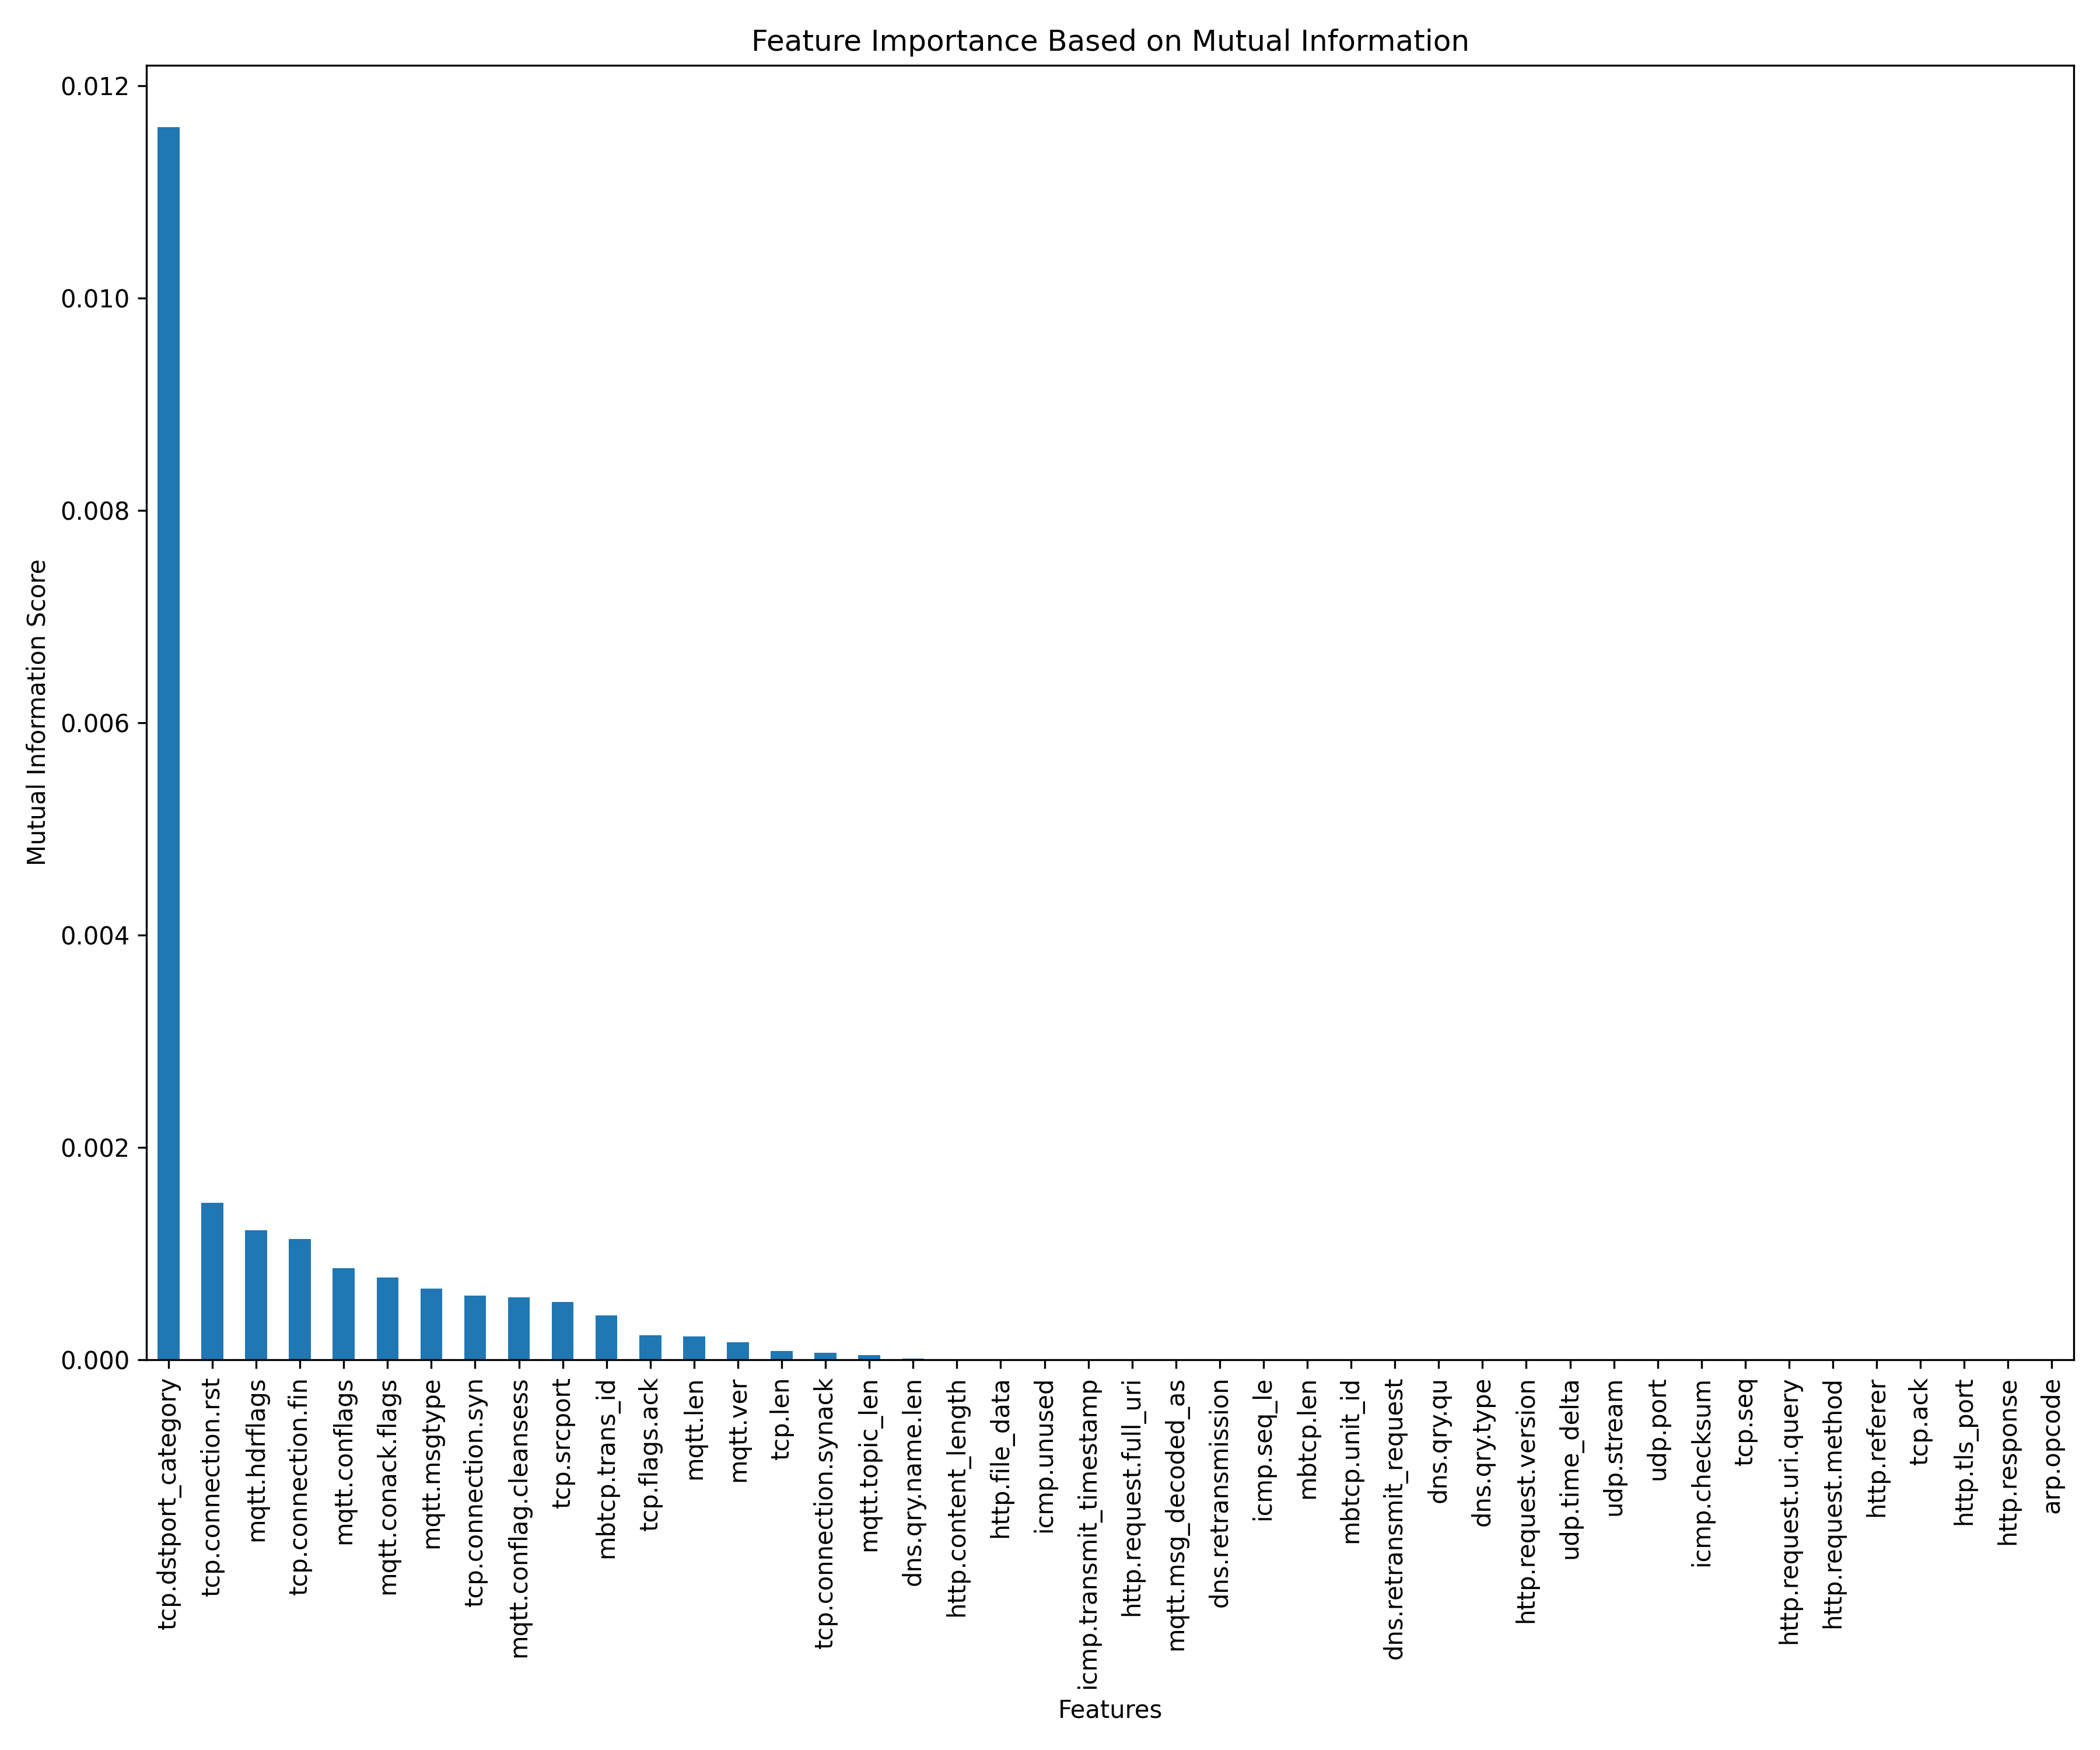
\includegraphics[width=\textwidth]{plots/mutual_information_scores.png}
\caption{Feature Importance Based on Mutual Information Scores}
\label{fig:mi_scores}
\end{figure}
\begin{longtable}{lrr}
\toprule
Feature & MI Score & Normalized Score \\
\midrule
tcp.dstport_category & 0.011610 & 1.000000 \\
tcp.connection.rst & 0.001473 & 0.126902 \\
mqtt.hdrflags & 0.001217 & 0.104795 \\
tcp.connection.fin & 0.001137 & 0.097904 \\
mqtt.conflags & 0.000860 & 0.074074 \\
mqtt.conack.flags & 0.000770 & 0.066322 \\
mqtt.msgtype & 0.000667 & 0.057422 \\
tcp.connection.syn & 0.000603 & 0.051967 \\
mqtt.conflag.cleansess & 0.000587 & 0.050531 \\
tcp.srcport & 0.000540 & 0.046512 \\
mbtcp.trans_id & 0.000417 & 0.035889 \\
tcp.flags.ack & 0.000230 & 0.019811 \\
mqtt.len & 0.000220 & 0.018949 \\
mqtt.ver & 0.000163 & 0.014068 \\
tcp.len & 0.000080 & 0.006891 \\
tcp.connection.synack & 0.000063 & 0.005455 \\
mqtt.topic_len & 0.000040 & 0.003445 \\
dns.qry.name.len & 0.000010 & 0.000861 \\
http.content_length & 0.000000 & 0.000000 \\
http.file_data & 0.000000 & 0.000000 \\
icmp.unused & 0.000000 & 0.000000 \\
icmp.transmit_timestamp & 0.000000 & 0.000000 \\
http.request.full_uri & 0.000000 & 0.000000 \\
mqtt.msg_decoded_as & 0.000000 & 0.000000 \\
dns.retransmission & 0.000000 & 0.000000 \\
icmp.seq_le & 0.000000 & 0.000000 \\
mbtcp.len & 0.000000 & 0.000000 \\
mbtcp.unit_id & 0.000000 & 0.000000 \\
dns.retransmit_request & 0.000000 & 0.000000 \\
dns.qry.qu & 0.000000 & 0.000000 \\
dns.qry.type & 0.000000 & 0.000000 \\
http.request.version & 0.000000 & 0.000000 \\
udp.time_delta & 0.000000 & 0.000000 \\
udp.stream & 0.000000 & 0.000000 \\
udp.port & 0.000000 & 0.000000 \\
icmp.checksum & 0.000000 & 0.000000 \\
tcp.seq & 0.000000 & 0.000000 \\
http.request.uri.query & 0.000000 & 0.000000 \\
http.request.method & 0.000000 & 0.000000 \\
http.referer & 0.000000 & 0.000000 \\
tcp.ack & 0.000000 & 0.000000 \\
http.tls_port & 0.000000 & 0.000000 \\
http.response & 0.000000 & 0.000000 \\
arp.opcode & 0.000000 & 0.000000 \\
\bottomrule
\caption{Mutual Information Scores for All Features}
\end{longtable}
\subsection{Principal Component Analysis}
Principal Component Analysis (PCA) was used to understand the variance contribution of each feature and dimensionality reduction potential.
\begin{figure}[ht]
\centering
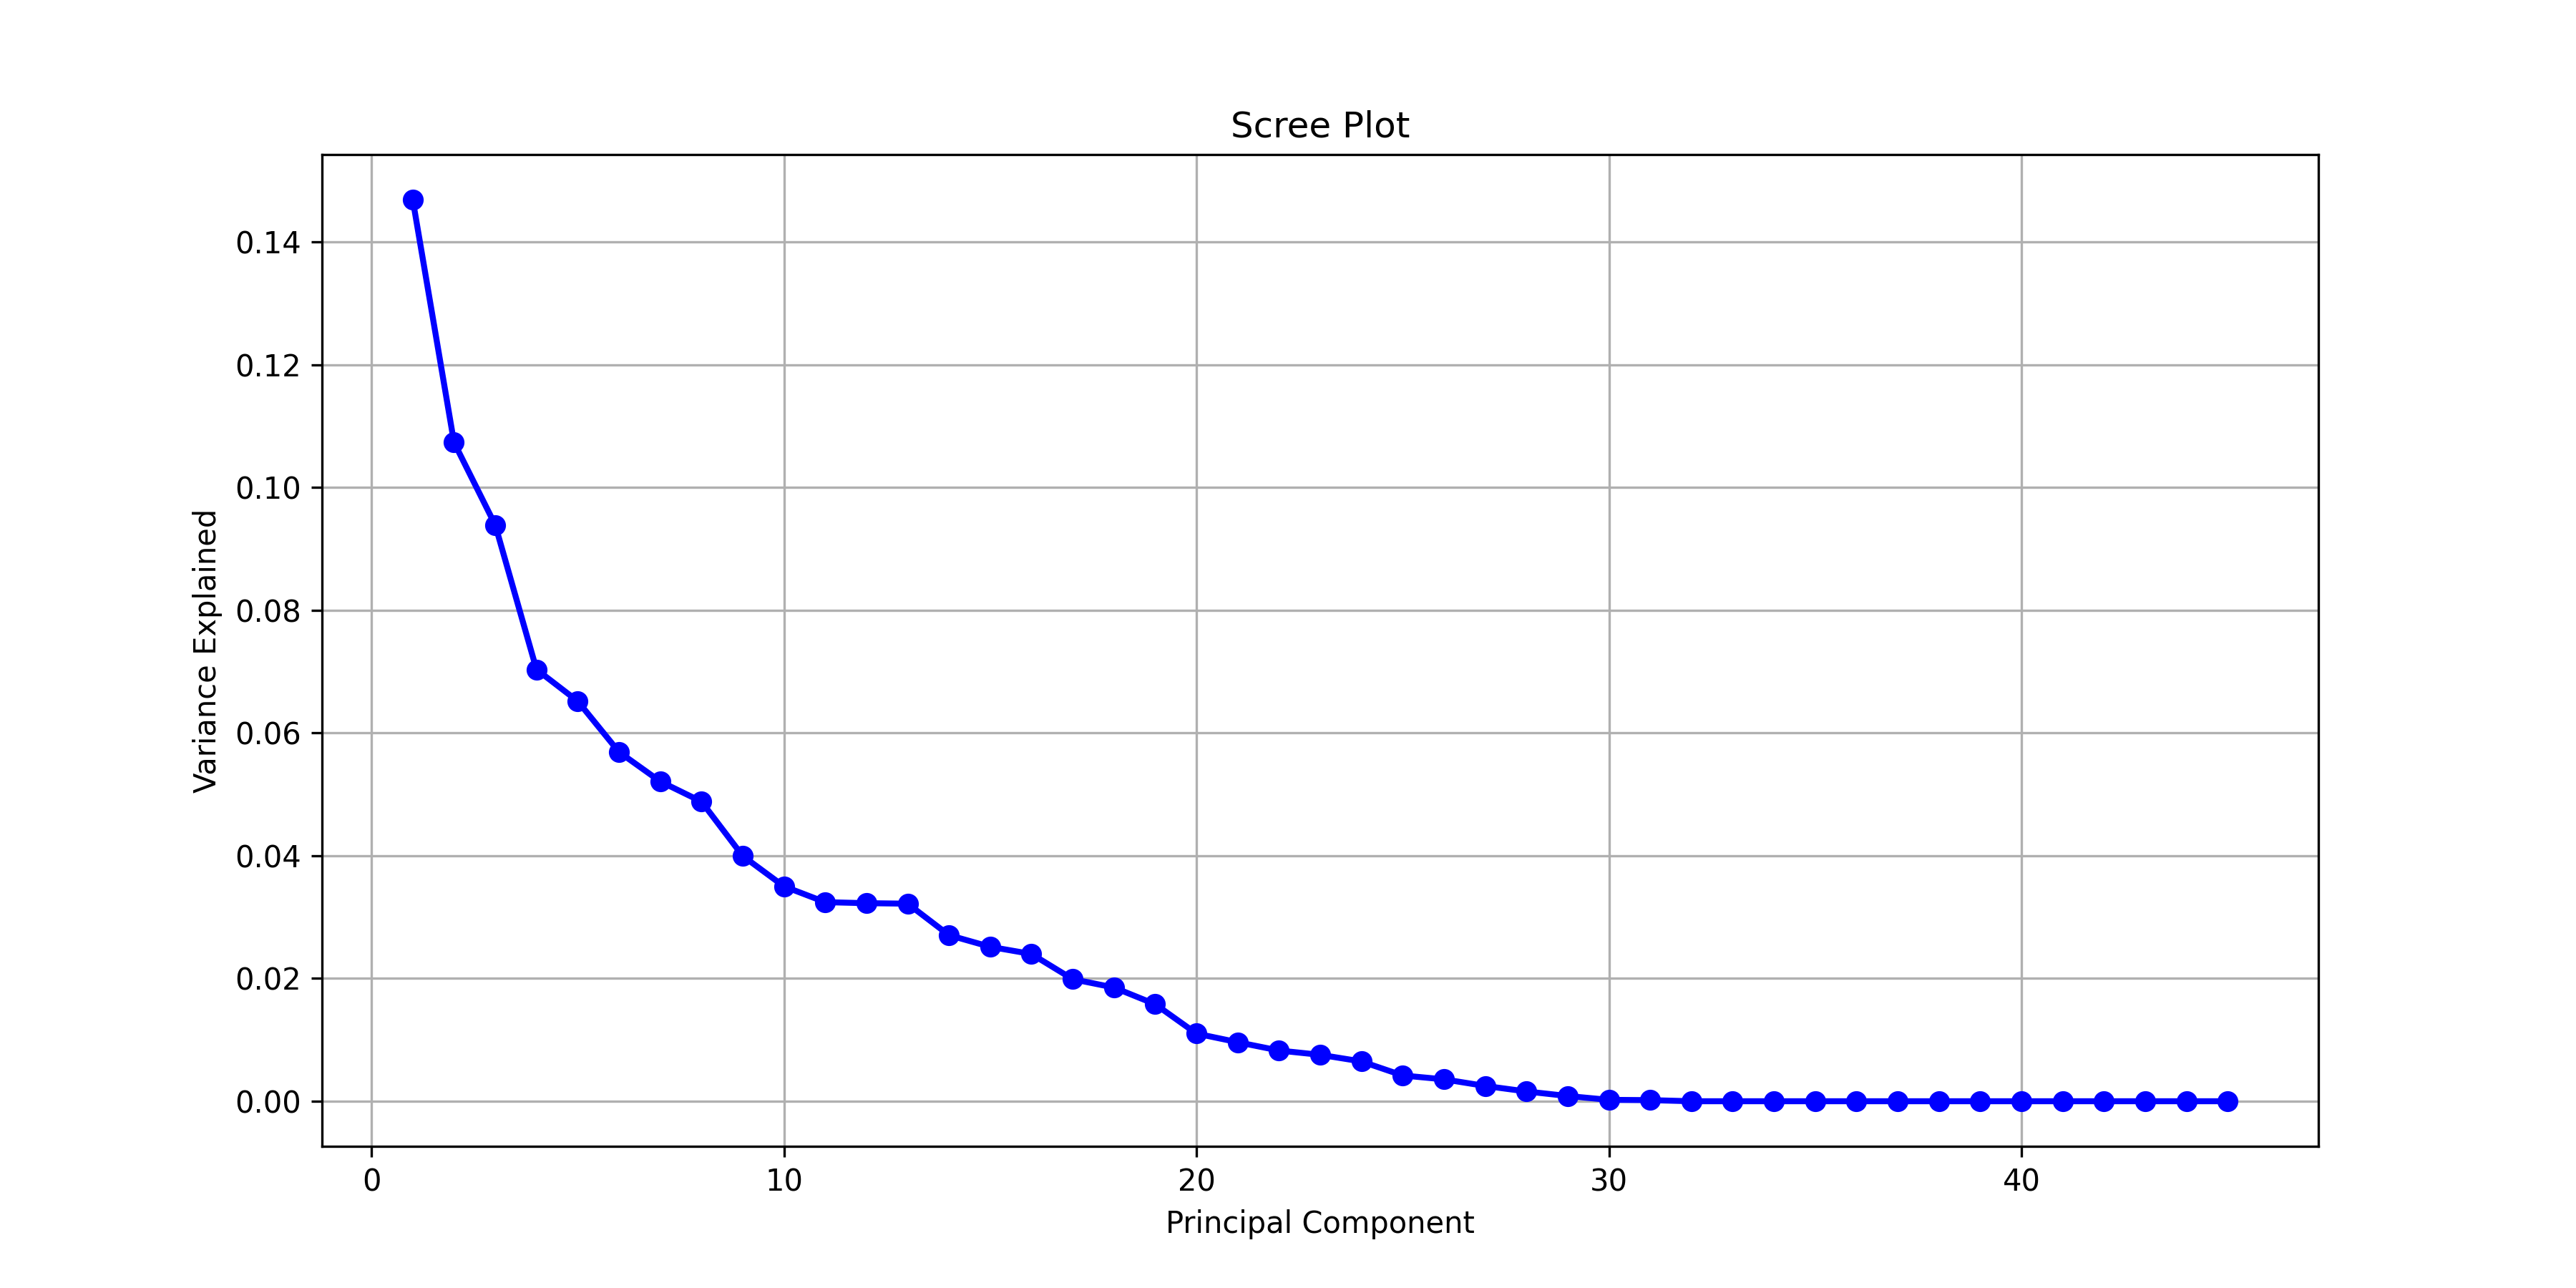
\includegraphics[width=0.8\textwidth]{plots/pca_scree_plot.png}
\caption{Scree Plot Showing Variance Explained by Each Principal Component}
\label{fig:pca_scree}
\end{figure}
\begin{figure}[ht]
\centering
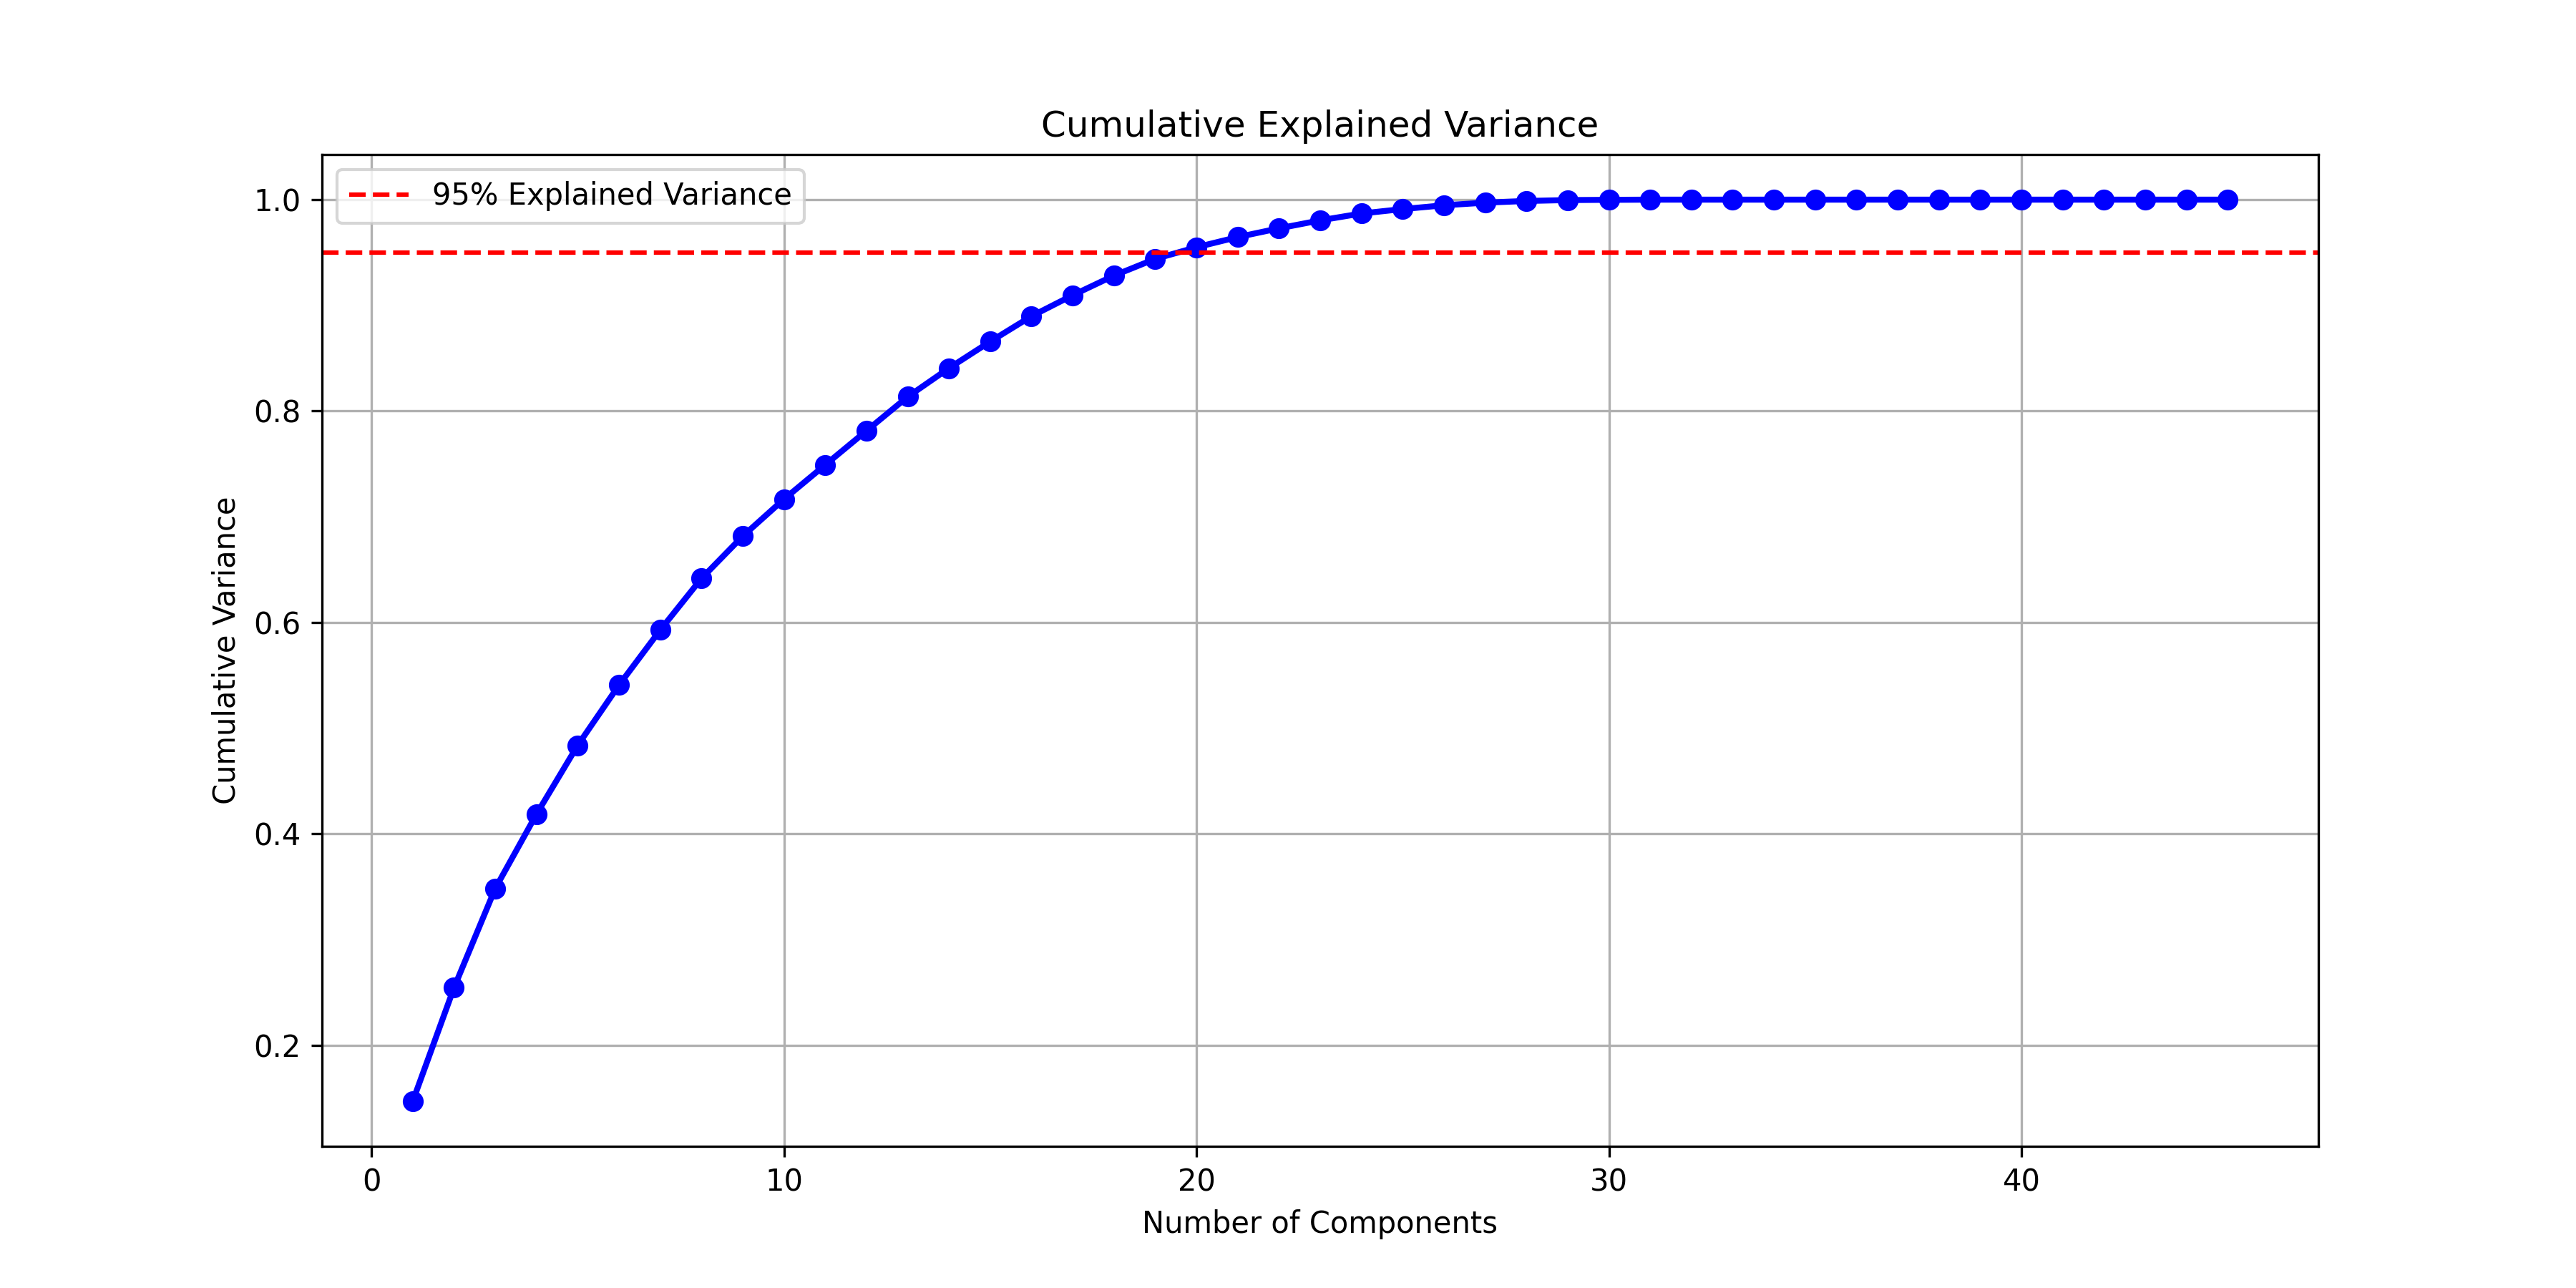
\includegraphics[width=0.8\textwidth]{plots/pca_cumulative_variance.png}
\caption{Cumulative Explained Variance by Principal Components}
\label{fig:pca_cumulative}
\end{figure}
Based on the PCA analysis, 20 components are needed to explain 95\% of the variance in the data.
\begin{figure}[ht]
\centering
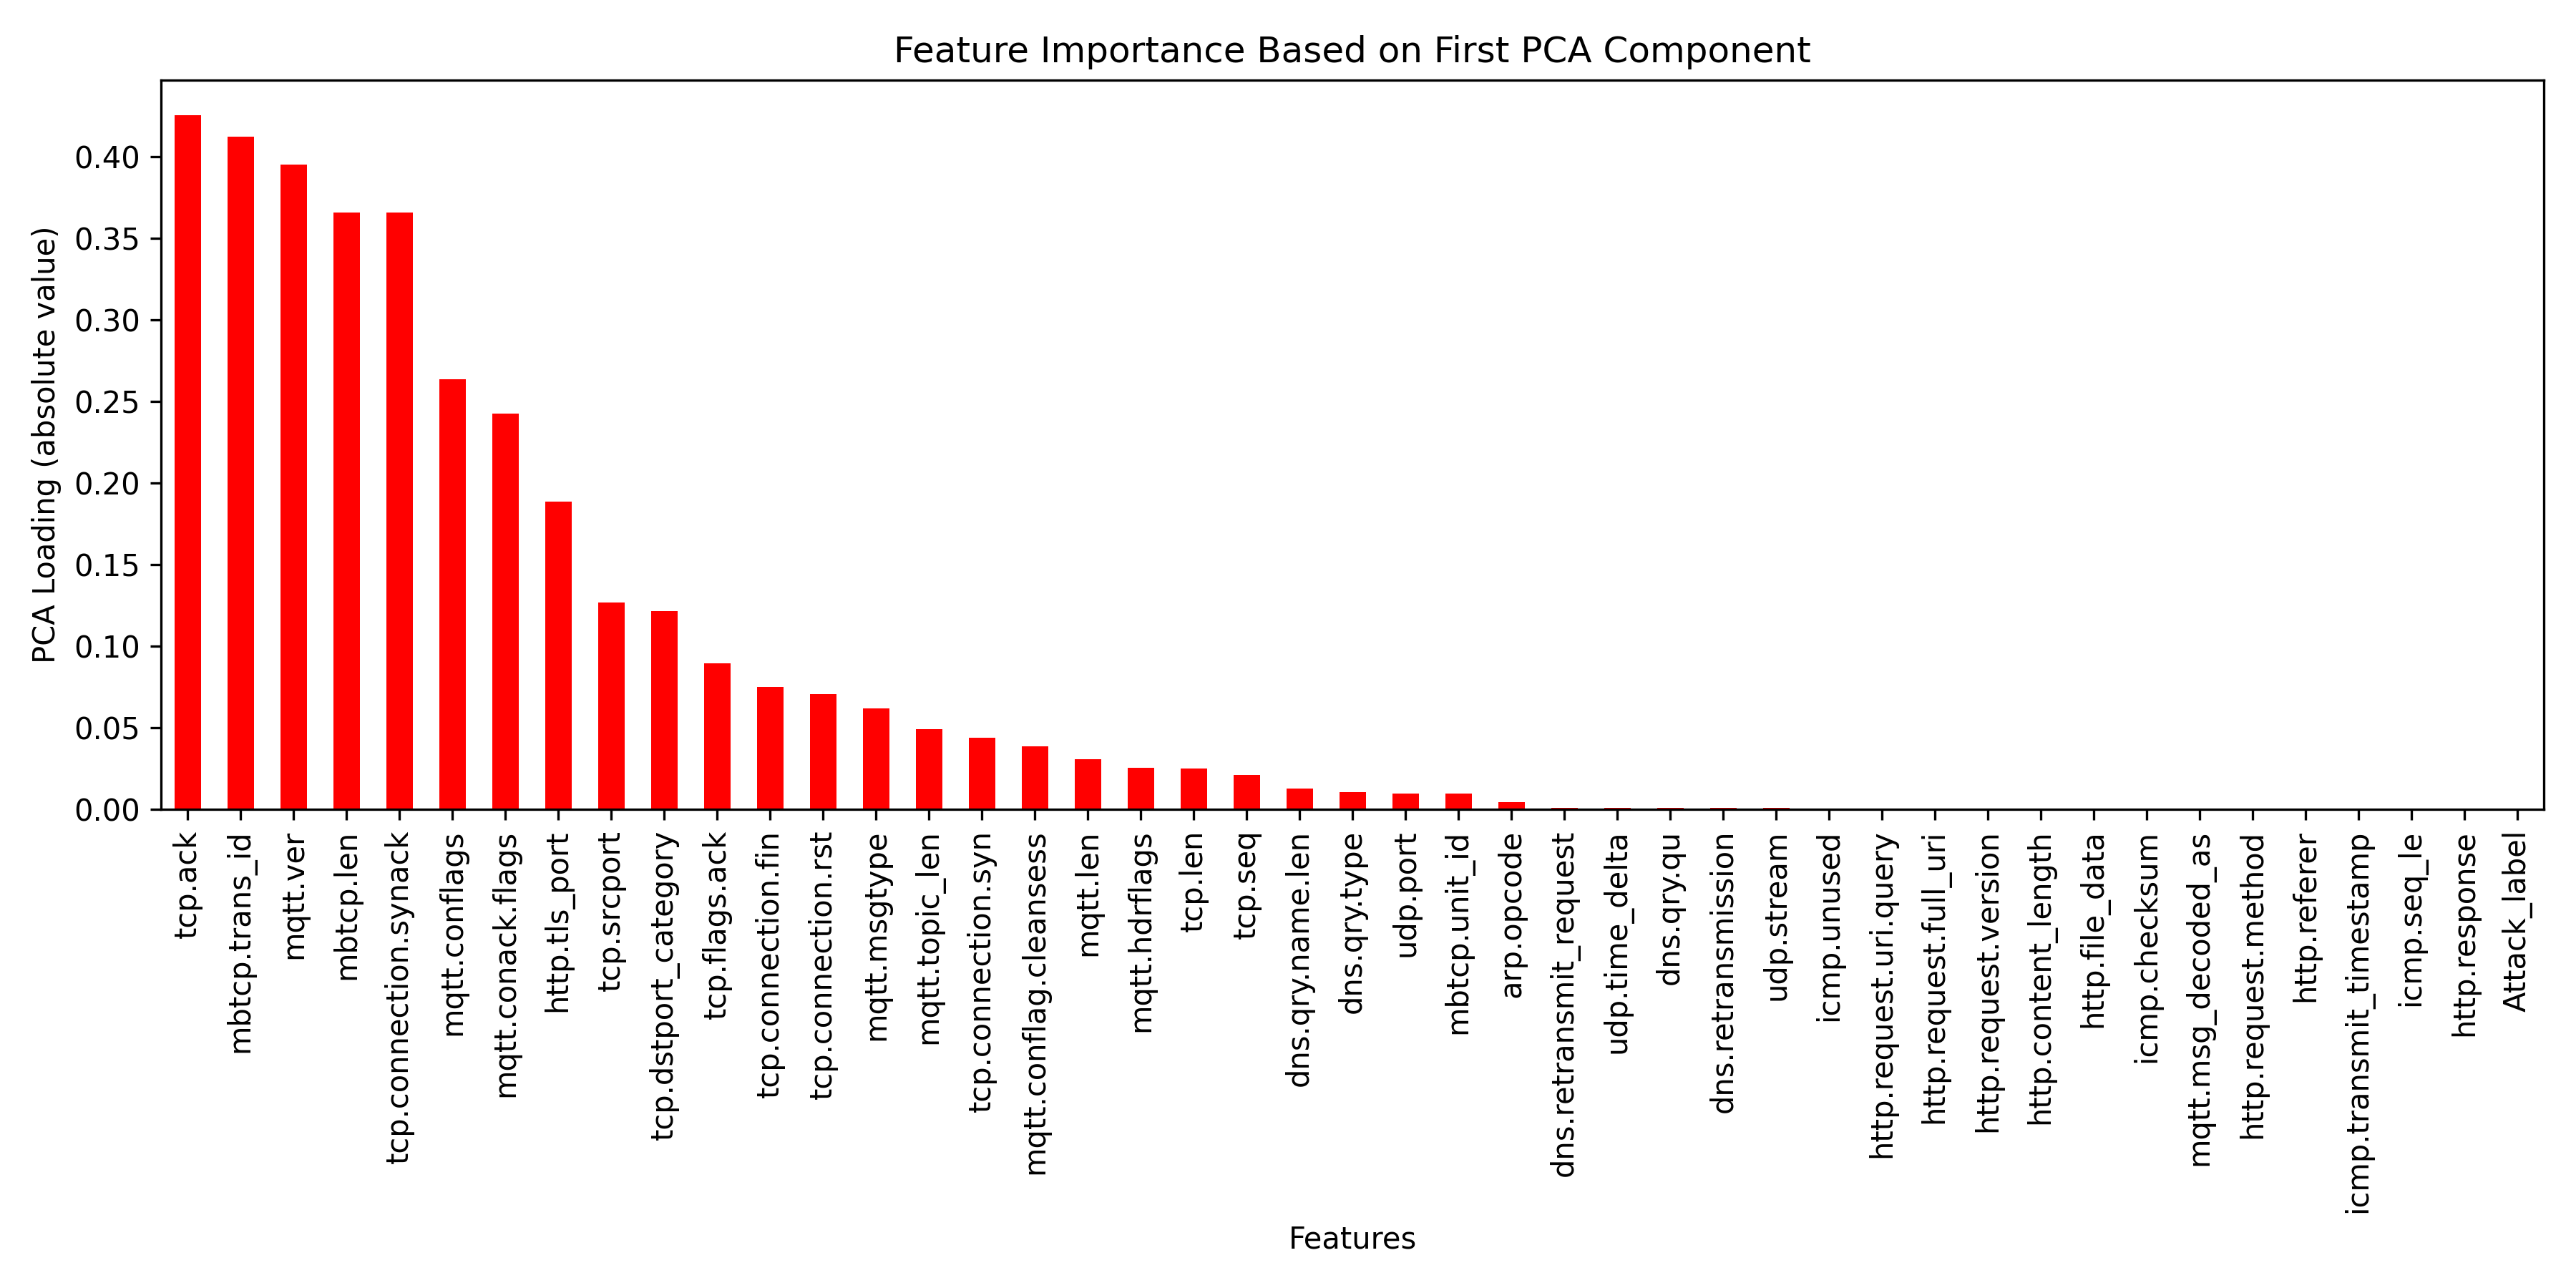
\includegraphics[width=\textwidth]{plots/pca_feature_importance.png}
\caption{Feature Importance Based on First PCA Component}
\label{fig:pca_importance}
\end{figure}
\begin{longtable}{lr}
\toprule
Feature & PCA Loading (abs) \\
\midrule
tcp.ack & 0.425450 \\
mbtcp.trans_id & 0.412198 \\
mqtt.ver & 0.395107 \\
mbtcp.len & 0.365724 \\
tcp.connection.synack & 0.365717 \\
mqtt.conflags & 0.263354 \\
mqtt.conack.flags & 0.242497 \\
http.tls_port & 0.188339 \\
tcp.srcport & 0.126433 \\
tcp.dstport_category & 0.121314 \\
tcp.flags.ack & 0.089360 \\
tcp.connection.fin & 0.074626 \\
tcp.connection.rst & 0.070290 \\
mqtt.msgtype & 0.061693 \\
mqtt.topic_len & 0.048812 \\
tcp.connection.syn & 0.043648 \\
mqtt.conflag.cleansess & 0.038428 \\
mqtt.len & 0.030429 \\
mqtt.hdrflags & 0.025446 \\
tcp.len & 0.024660 \\
tcp.seq & 0.020645 \\
dns.qry.name.len & 0.012592 \\
dns.qry.type & 0.010411 \\
udp.port & 0.009497 \\
mbtcp.unit_id & 0.009444 \\
arp.opcode & 0.004178 \\
dns.retransmit_request & 0.000795 \\
udp.time_delta & 0.000745 \\
dns.qry.qu & 0.000539 \\
dns.retransmission & 0.000474 \\
udp.stream & 0.000462 \\
icmp.transmit_timestamp & 0.000000 \\
icmp.checksum & 0.000000 \\
http.content_length & 0.000000 \\
http.request.method & 0.000000 \\
http.request.full_uri & 0.000000 \\
http.request.version & 0.000000 \\
http.file_data & 0.000000 \\
http.request.uri.query & 0.000000 \\
mqtt.msg_decoded_as & 0.000000 \\
http.referer & 0.000000 \\
icmp.unused & 0.000000 \\
icmp.seq_le & 0.000000 \\
http.response & 0.000000 \\
\bottomrule
\caption{PCA-based Feature Importance Scores}
\end{longtable}
\subsection{Combined Feature Selection}
We combined the results from Mutual Information and PCA to obtain a more robust feature selection. Features were selected based on a combined score that gives 70\% weight to MI and 30\% weight to PCA importance.
\begin{longtable}{lrrr}
\toprule
Feature & MI Score & PCA Loading & Combined Score \\
\midrule
tcp.dstport_category & 0.011610 & 0.121314 & 0.785543 \\
mbtcp.trans_id & 0.000417 & 0.412198 & 0.315778 \\
tcp.ack & 0.000000 & 0.425450 & 0.300000 \\
mqtt.ver & 0.000163 & 0.395107 & 0.288452 \\
tcp.connection.synack & 0.000063 & 0.365717 & 0.261698 \\
mbtcp.len & 0.000000 & 0.365724 & 0.257885 \\
mqtt.conflags & 0.000860 & 0.263354 & 0.237552 \\
mqtt.conack.flags & 0.000770 & 0.242497 & 0.217419 \\
tcp.connection.rst & 0.001473 & 0.070290 & 0.138396 \\
http.tls_port & 0.000000 & 0.188339 & 0.132805 \\
tcp.srcport & 0.000540 & 0.126433 & 0.121710 \\
tcp.connection.fin & 0.001137 & 0.074626 & 0.121154 \\
mqtt.hdrflags & 0.001217 & 0.025446 & 0.091299 \\
mqtt.msgtype & 0.000667 & 0.061693 & 0.083697 \\
tcp.flags.ack & 0.000230 & 0.089360 & 0.076879 \\
tcp.connection.syn & 0.000603 & 0.043648 & 0.067154 \\
mqtt.conflag.cleansess & 0.000587 & 0.038428 & 0.062469 \\
mqtt.topic_len & 0.000040 & 0.048812 & 0.036831 \\
mqtt.len & 0.000220 & 0.030429 & 0.034721 \\
tcp.len & 0.000080 & 0.024660 & 0.022212 \\
tcp.seq & 0.000000 & 0.020645 & 0.014558 \\
dns.qry.name.len & 0.000010 & 0.012592 & 0.009482 \\
dns.qry.type & 0.000000 & 0.010411 & 0.007341 \\
udp.port & 0.000000 & 0.009497 & 0.006697 \\
mbtcp.unit_id & 0.000000 & 0.009444 & 0.006660 \\
arp.opcode & 0.000000 & 0.004178 & 0.002946 \\
dns.retransmit_request & 0.000000 & 0.000795 & 0.000560 \\
udp.time_delta & 0.000000 & 0.000745 & 0.000525 \\
dns.qry.qu & 0.000000 & 0.000539 & 0.000380 \\
dns.retransmission & 0.000000 & 0.000474 & 0.000335 \\
\bottomrule
\caption{Top 30 Features Based on Combined Importance Score}
\end{longtable}
\subsection{Conclusion}
Based on our analysis, we identified 13 features as important for anomaly detection. These features will be used in the Layer 1 (Autoencoder-VAE) of the GORK AI system.
\paragraph{Selected Features:}
\begin{itemize}
\item tcp.dstport_category
\item mbtcp.trans_id
\item tcp.ack
\item mqtt.ver
\item tcp.connection.synack
\item mbtcp.len
\item mqtt.conflags
\item mqtt.conack.flags
\item tcp.connection.rst
\item http.tls_port
\item tcp.srcport
\item tcp.connection.fin
\item mqtt.hdrflags
\end{itemize}
\end{document}
